\documentclass[a4paper]{ctexart}

\usepackage{geometry, fancyhdr, amsmath, booktabs, graphicx, wrapfig, textcomp}
\usepackage{cmap}
%\usepackage{syntonly}
%\syntaxonly

\geometry{left=1.25in, right=1.25in, top=1in, bottom=1in}
\pagestyle{fancy}
\fancyhead[L]{乙酸乙酯皂化反应速率常数的测定}
\fancyhead[R]{2020.11.3}

\begin{document}
\section*{实验十四\ 乙酸乙酯皂化反应速率常数的测定}


	\begin{center}
	匡亚明学院\ 霍然 171240008
	\end{center}


	\subsection*{一、实验目的}
		\begin{enumerate}
			\item 掌握测定化学反应速率常数的一种物理方法——电导法。
			\item 掌握二级反应的特点,掌握用图解法求二级反应的速率常数。
			\item 掌握DDS-11A(T)型电导率仪的使用方法。
		\end{enumerate}
		
		
	\subsection*{二、实验原理}
		反应速率与反应物浓度二次方成正比的反应称为二级反应。对于二级反应A + B $\longrightarrow$ C,
		如果反应物A与反应物B起始浓度相同,均为$c_a$,则反应速率的表达式为
		\begin{equation}
			\frac{\mathrm{d}c_x}{\mathrm{d}t}=k\left(c_a-c_x\right)^2
		\end{equation}
		其中$c_x$为时间 $t$ 时反应物浓度的减小,上式定积分得
		\begin{equation}
			k=\frac{1}{tc_a}\cdot\frac{c_x}{c_a-c_x}
		\end{equation}
		以$\dfrac{c_x}{c_a-c_x}-t$作图若所得为直线,则反应为二级反应,且可从直线的斜率求出速率常数$k$。
		所以在反应进行过程中,只要能够测出反应物或产物的浓度,即可求得该反应的速率常数$k$。
		
		如果知道两个不同温度下的速率常数$k_{T_1}$和$k_{T_2}$,
		则可按Arrhenius公式计算出反应在该温度范围内的平均活化能$E_a$:
		\begin{equation}
			E_a=ln\frac{k_{T_2}}{k_{T_1}}\times R\left(\frac{T_1\cdot T_2}{T_2-T_1}\right)
		\end{equation}
		
		乙酸乙酯的皂化反应是二级反应,其反应式为
		\begin{center}
			CH$_3$COOC$_2$H$_5$ + OH$^-$ $\longrightarrow$ CH$_3$COO$^-$ +C$_2$H$_5$OH
		\end{center}
		OH$^-$电导率大,CH$_3$COO$^-$电导率小。因此,在反应进行过程中,电导率大的OH$^-$逐渐为电导率小的
		CH$_3$COO$^-$所取代,溶液电导率有显著降低。对稀溶液而言,强电解质的电导率$\kappa$与其浓度成正比,
		而且溶液的总电导率就等于组成该溶液的电解质电导率之和。如果乙酸乙酯皂化在稀溶液下反应,就存在如下关系
		式:
		\begin{gather}
			\kappa_0=A_1c_a \\
			\kappa_\infty=A_2c_a \\
			\kappa_t=A_1\left(c_a-c_x\right)+A_2c_x
		\end{gather}
		其中$A_1$、$A_2$分别是与温度、电解质性质、溶剂等因素有关的比例常数;$\kappa_0$、$\kappa_\infty$
		分别为反应时间$t=0$和$t=\infty$时溶液的总电导率;$\kappa_t$为反应时间$t=t$时溶液的总电导率。
		由以上三式得
		\begin{equation}
			c_x=\left(\frac{\kappa_0-\kappa_t}{\kappa_0-\kappa_\infty}\right)\cdot c_a
		\end{equation}
		代入(1)式得
		\begin{equation}
			k=\frac{1}{t\cdot c_a}\left(\frac{\kappa_0-\kappa_t}{\kappa_t-\kappa_\infty}\right)
		\end{equation}
		重新排列得
		\begin{equation}
			\kappa_t=\frac{1}{c_ak}\frac{\kappa_0-\kappa_t}{t}+\kappa_\infty
		\end{equation}
		因此,以$\kappa_t-\dfrac{\kappa_0-\kappa_t}{t}$作图为一条直线即为二级反应,从直线的斜率可求出
		速率常数$k$。由两个不同温度下测得的速率常数$k_{T_1}$、$k_{T_2}$,
		可计算出该反应在该温度范围内的平均活化能$E_a$。
		
		
	\subsection*{三、仪器与药品}
		DDS-11A(T)型电导率仪(附DIS型铂黑电极)1台;计时器1支;恒温槽1套;双管式电导池2只;
		25 mL胖肚移液管3支;50 mL烧杯1只;100 mL容量瓶1只;称量瓶($\phi$25 mm $\times$23 mm)1只
		
		CH$_3$COOC$_2$H$_5$(AR);0.0200 mol/L NaOH溶液;电导水
		
		
	\subsection*{四、实验步骤}\par
		\begin{wrapfigure}{r}{4cm}
			\centering
			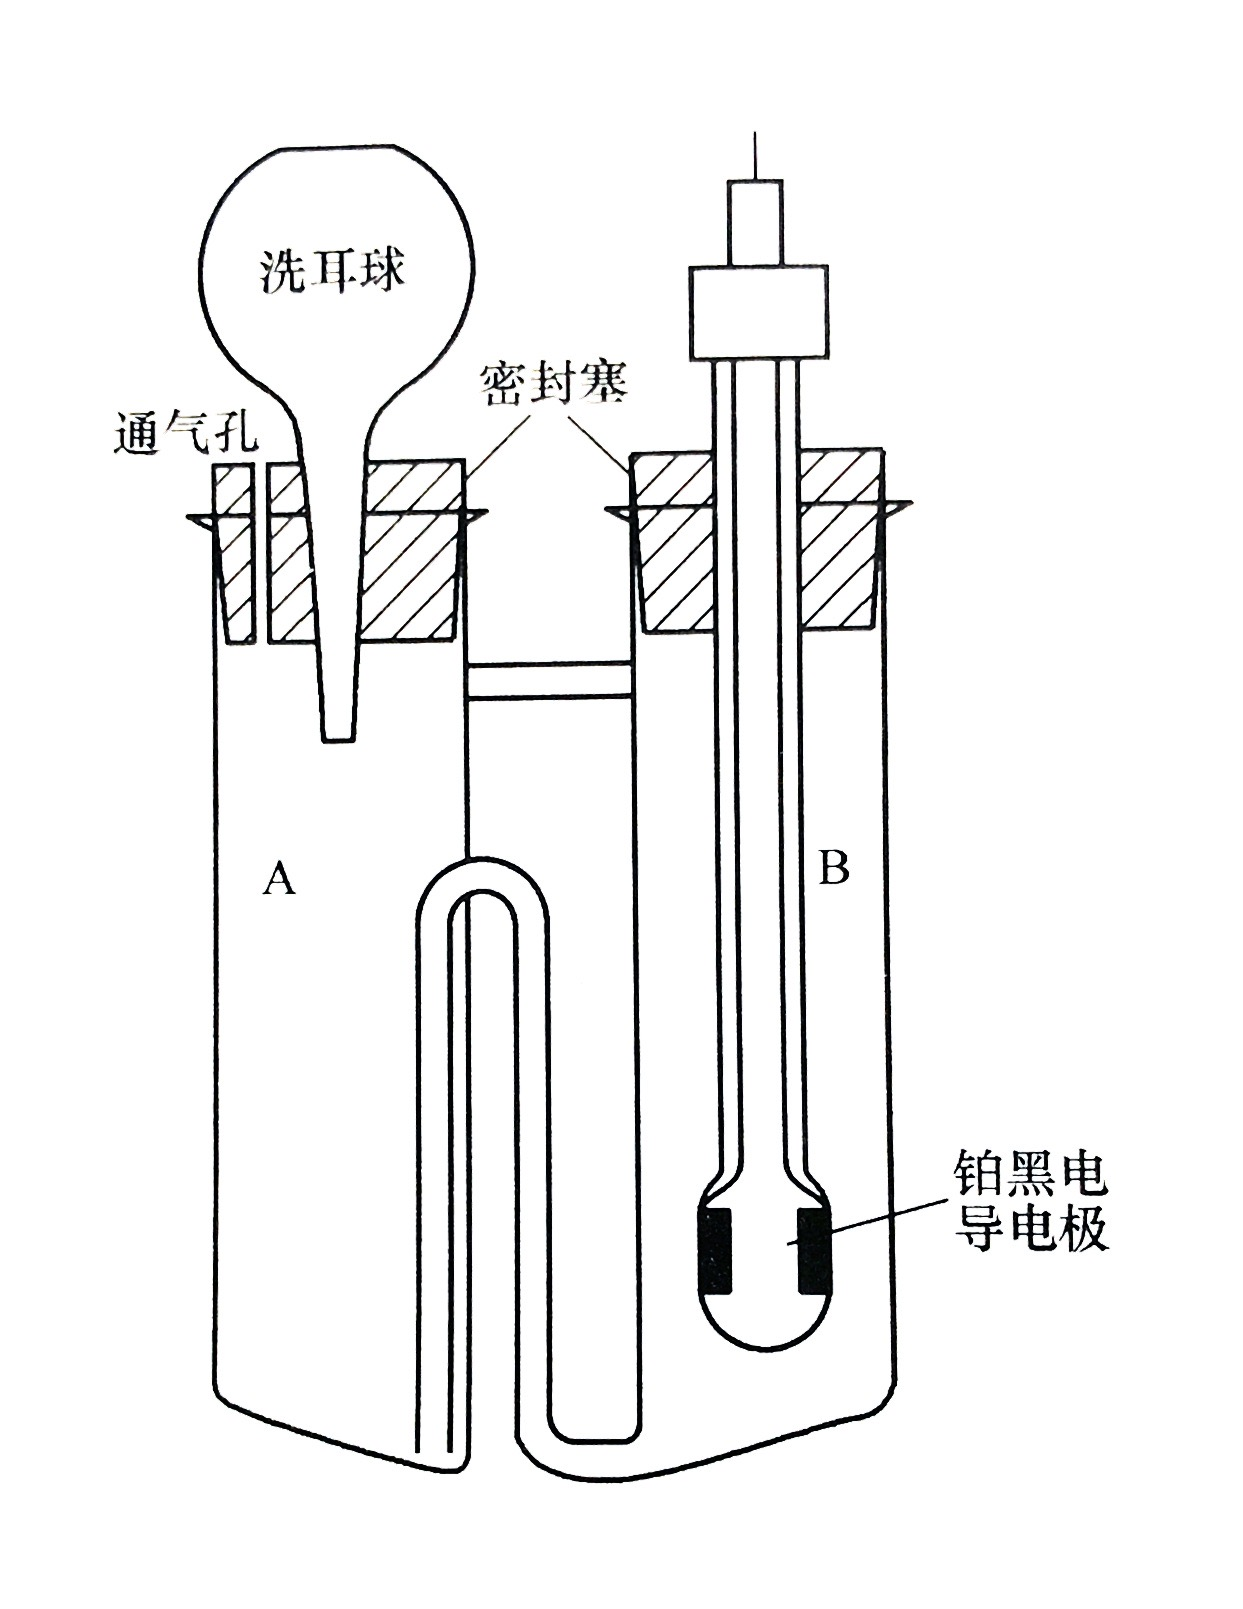
\includegraphics[width=10em]{1.jpeg}
			\caption{双管式电导池}
		\end{wrapfigure}
		\  \\
		1. 调节恒温槽为298.2 K。用电导水配置0.0200 mol/L CH$_3$COOC$_2$H$_5$ 100mL。\\[6pt]
		2. $\kappa_0$的测定。取10 mL电导水和10 mL 0.0200 mol/L NaOH溶液,分别加到干燥洁净的双管式电导池的
		A管和B管中,恒温10 min。用洗耳球吸、压多次使溶液充分混合均匀后将溶液压到双管式电导池的B管中,
		将经电导水淋洗并吸干其外侧表面的电导电极插入溶液中,
		用DDS-11A(T)型电导率仪测定上述已恒温的NaOH溶液,所得电导率即为$\kappa_0$。\\[6pt]
		3. $\kappa_t$的测定。分别在另一双管式电导池的A管和B管中加入10 mL 0.0200 mol/L
		CH$_3$COOC$_2$H$_5$和10 mL 0.0200 mol/L NaOH溶液,恒温10 min。用前述方法混合反应溶液
		并测定电导率。必须在两反应液一接触时就启动计时器记录反应时间(注意计时器一经打开切勿按停,
		直至实验全部结束)。当反应进行6 min时测电导率一次,并在9 min、12 min、15 min、20 min、25 min、
		30 min、35 min、40 min、50 min、60 min时分别测电导率$\kappa_t$一次,记录$\kappa_t$和时间$t$。\\[6pt]
		4. 调节恒温槽温度为308.2 K,重复上述实验步骤测定其$\kappa_0$和$\kappa_t$。$\kappa_t$是在反应
		进行至4 min、6 min、8 min、10 min、12 min、15 min、18 min、21 min、24 min、27 min、30 min时测定。
		
		
	\subsection*{五、数据记录与处理}
		T = 25.000 \textcelsius 时$t$、$K_t$与$\dfrac{K_0-K_t}{t}$的值见表1,用$K_t$对$\dfrac{K_0-K_t}{t}$作图并拟合的结果见图2。\par
		\begin{table}[htb]
			\caption{T = 25.000 \textcelsius 时的实验数据记录表}
			\begin{center}
				\begin{tabular}{p{6em}p{12em}p{16em}}
				\toprule
				$t$ (min) & $K_t$ ($\mu$S $\cdot$ cm$^{-1}$)
				& $\dfrac{K_0-K_t}{t}$ ($\mu$S$\cdot$cm$^{-1}$ $\cdot$ min$^{-1}$) \\
				\midrule
				0 & 2250 & / \\
				6 & 1865 & 64.2 \\
				9 & 1756 & 54.9 \\
				12 & 1667 & 48.6 \\
				15 & 1598 & 43.5 \\
				20 & 1508 & 37.1 \\
				25 & 1438 & 32.5 \\
				30 & 1382 & 28.9 \\
				35 & 1337 & 26.1 \\
				40 & 1302 & 23.7 \\
				50 & 1244 & 20.1 \\
				60 & 1202 & 17.5 \\ 
				\bottomrule
				\end{tabular}
			\end{center}
			\label{default}
		\end{table}
		\begin{figure}[htb]
			\begin{center}
			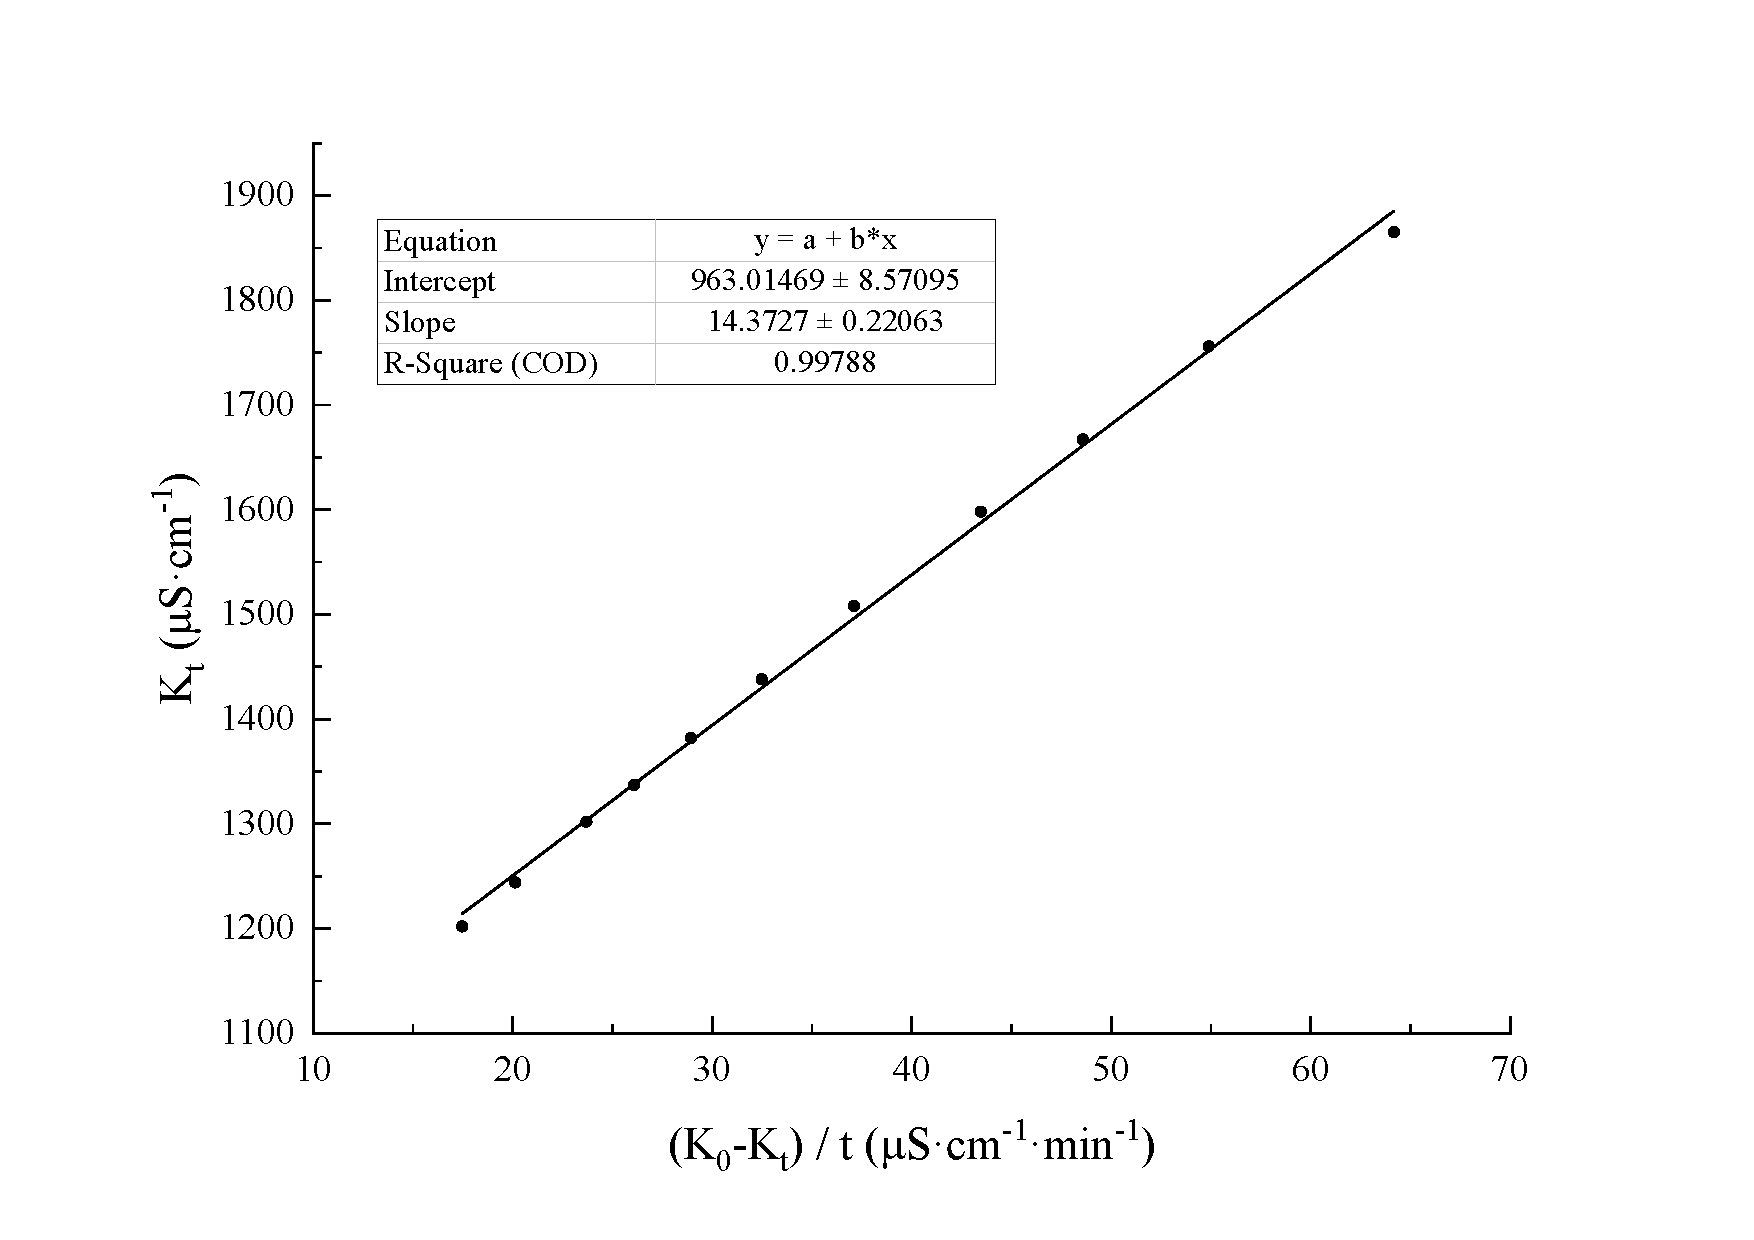
\includegraphics[width=36em]{T=25.pdf}
			\caption{T = 25.000 \textcelsius 时的$\kappa_t-\dfrac{\kappa_0-\kappa_t}{t}$图}
			\label{}
			\end{center}
		\end{figure}
		\clearpage
		由斜率$b=14.4$ min可得反应速率常数
		\begin{align*}
			k&=\frac{1}{c_ab} \\
			&=\frac{1}{0.0100\text{ mol·L}^{-1}\times14.4\text{ min}} \\
			&=6.94\text{ mol}^{-1}\cdot \text{ dm}^3\cdot \text{min}^{-1}
		\end{align*}

		T = 35.000 \textcelsius 时$t$、$K_t$与$\dfrac{K_0-K_t}{t}$的值见表2,用$K_t$对$\dfrac{K_0-K_t}{t}$作图并拟合的结果见图3。\par
		\begin{table}[htb]
			\caption{T = 35.000 \textcelsius 时的实验数据记录表}
			\begin{center}
				\begin{tabular}{p{6em}p{12em}p{16em}}
				\toprule
				$t$ (min) & $K_t$ ($\mu$S $\cdot$ cm$^{-1}$)
				& $\dfrac{K_0-K_t}{t}$ ($\mu$S$\cdot$cm$^{-1}$ $\cdot$ min$^{-1}$) \\
				\midrule
				0 &  2260 & / \\
				4 & 1821 & 110 \\
				6 & 1690 & 95.0\\
				8 & 1602 & 82.2 \\
				10 & 1532 & 72.8 \\
				12 & 1473 & 65.6 \\
				15 & 1407 & 56.9 \\
				18 & 1357 & 50.2 \\
				21 & 1316 & 45.0 \\
				24 & 1282 & 40.8 \\
				27 & 1255 & 37.2 \\
				30 & 1231 & 34.3 \\
				\bottomrule
				\end{tabular}
			\end{center}
			\label{default}
		\end{table}
		\begin{figure}[htb]
			\begin{center}
			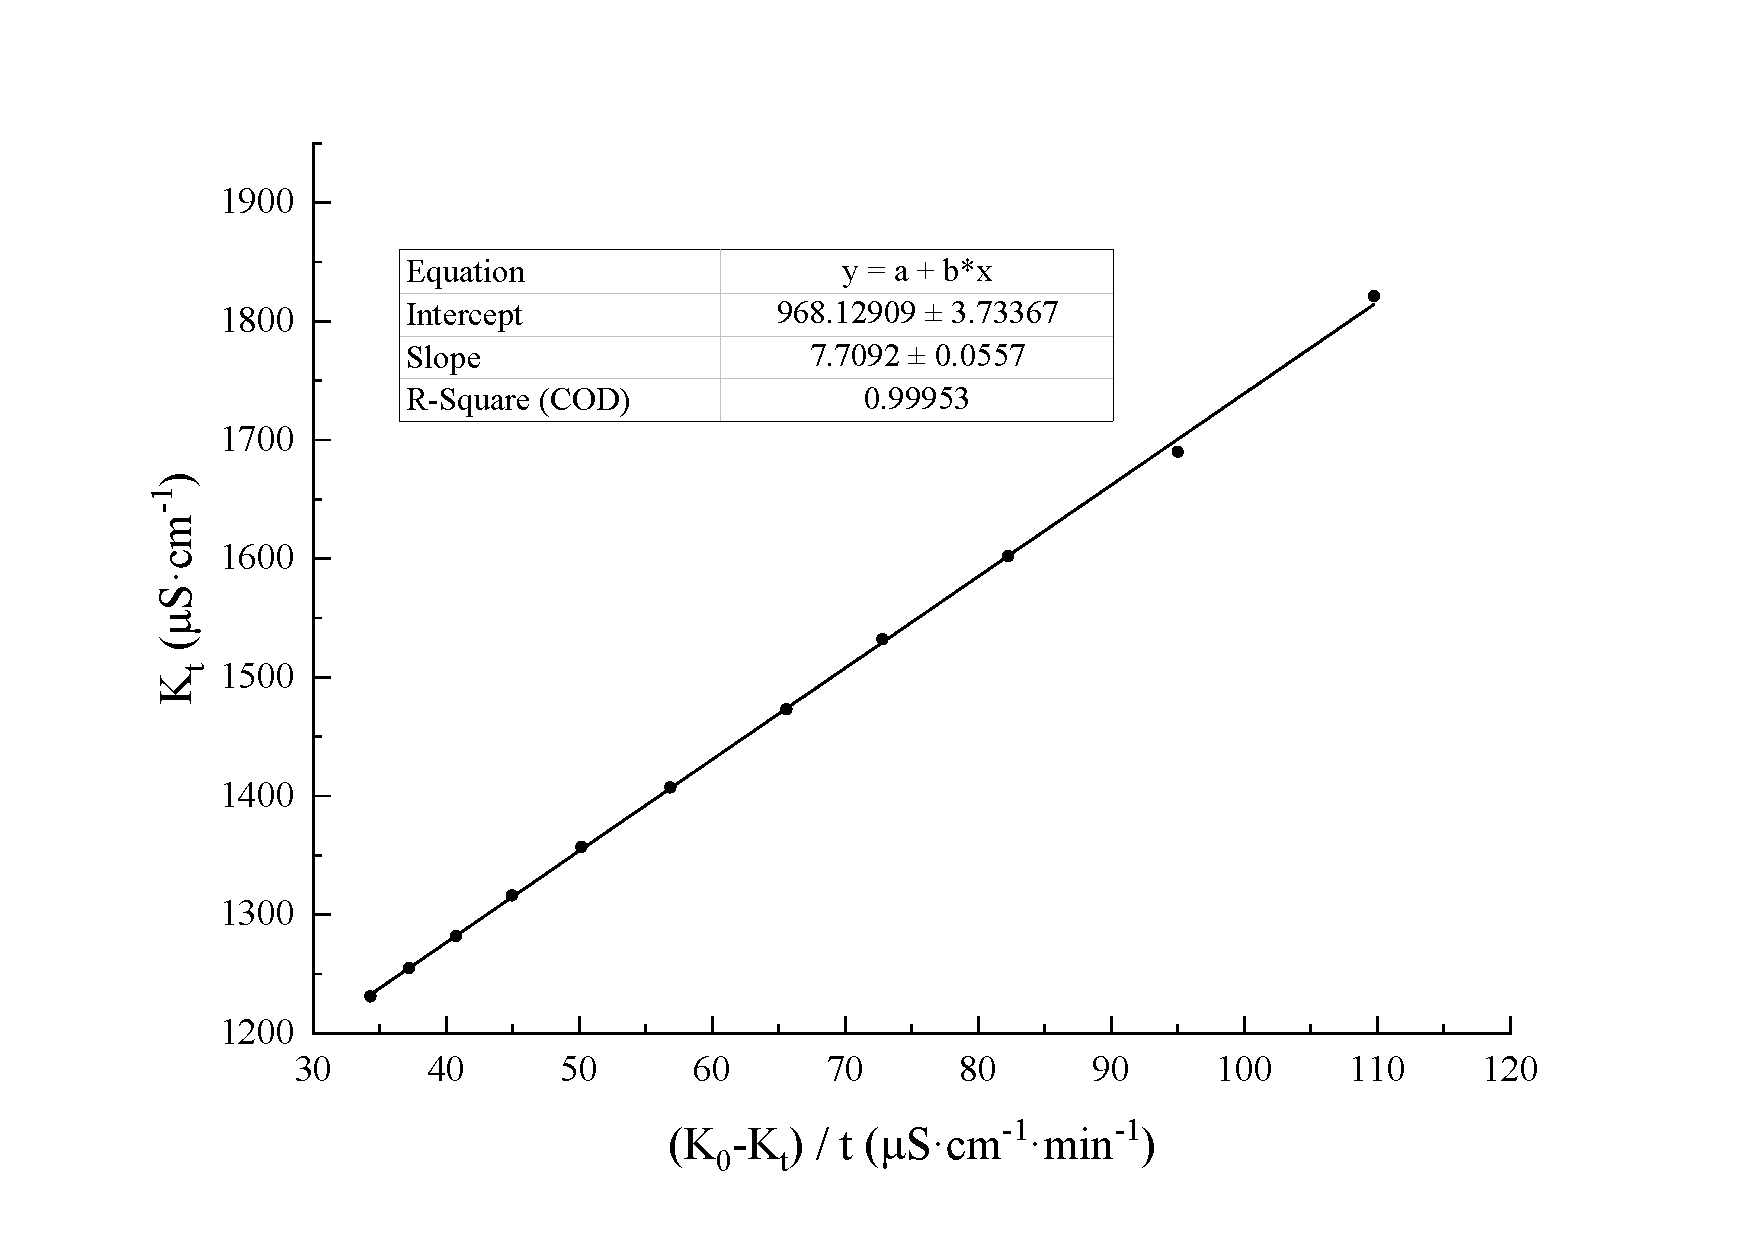
\includegraphics[width=30em]{T=35.pdf}
			\caption{T = 35.000 \textcelsius 时的$\kappa_t-\dfrac{\kappa_0-\kappa_t}{t}$图}
			\label{}
			\end{center}
		\end{figure}
		由斜率$b=7.71$ min可得反应速率常数
		\begin{align*}
			k&=\frac{1}{c_ab} \\
			&=\frac{1}{0.0100\text{ mol·L}^{-1}\times7.71\text{ min}} \\
			&=13.0\text{ mol}^{-1}\cdot \text{ dm}^3\cdot \text{min}^{-1}
		\end{align*}
		
		由Arrhenius公式计算出反应在该温度范围内的平均活化能$E_a$:
		\begin{align*}
			E_a	&=ln\frac{k_{T_2}}{k_{T_1}}\times R\left(\frac{T_1\cdot T_2}{T_2-T_1}\right) \\
				&=ln\frac{13.0}{6.94}\times 8.314\times 10^{-3}\left(\frac{298.15\times 308.15}{308.15-298.15}\right)\text{ kJ/mol}\\
				&=47.9\text{ kJ/mol}
		\end{align*}
		
	\subsection*{六、思考题}
		\begin{enumerate}
		\item 如果NaOH溶液和CH$_3$COOC$_2$H$_5$溶液起始浓度不相等,如何计算$k$值?\par
		当两种反应物起始浓度不相等时(即$c_a\neq c_b$时)反应速率方程变为
		\begin{equation}
			\frac{\mathrm{d}c_x}{\mathrm{d}t}=k\left(c_a-c_x\right)\left(c_b-c_x\right)
		\end{equation}
		对上式定积分得
		\begin{equation}
			k = \frac{1}{t(c_b-c_a)}ln\frac{c_a(c_b-c_x)}{c_b(c_a-c_x)}
		\end{equation}
		以$ln\dfrac{c_a(c_b-c_x)}{c_b(c_a-c_x)}$对时间$t$作图,即可从拟合的直线斜率求出$k$。\\[6pt]
		若想用电导法测定反应速率常数$k$,则首先应确定两种反应物浓度的大小关系。设NaOH起始浓度为$c_a$,
		CH$_3$COOC$_2$H$_5$起始浓度为$c_b$,若$c_a<c_b$,则式(4)--(7)仍成立,可直接代入(11)式;
		若$c_a>c_b$,则式(4)--(7)将变为
		\begin{gather}
			\kappa_0=A_1c_a \\
			\kappa_\infty=A_2c_b+A_1(c_a-c_b) \\
			\kappa_t=A_1\left(c_a-c_x\right)+A_2c_x
		\end{gather}
		由以上三式得
		\begin{equation}
			c_x=\left(\frac{\kappa_0-\kappa_t}{\kappa_0-\kappa_\infty}\right)\cdot c_b
		\end{equation}
		将其带入(11)式即可。此法需要人为测定$\kappa_\infty$的值。
		\item 如果NaOH溶液和CH$_3$COOC$_2$H$_5$溶液为浓溶液,能否用此法求$k$值?为什么?\par
		不能。因为本实验中用测电导率代替测反应物浓度的前提是“稀溶液中,强电解质的电导率与其浓度成正比,
		且溶液的总电导率等于组成该溶液的电解质电导率之和”。当稀溶液的前提不成立时,自然不能用此法求$k$值。
		\end{enumerate}
		
	\subsection*{七、讨论}
	查阅文献得25~\textcelsius 时乙酸乙酯皂化反应的速率常数$k$为
	$6.42\text{ mol}^{-1}\cdot \text{ dm}^3\cdot \text{min}^{-1}$,35~\textcelsius 时$k$为
	$10.5\text{ mol}^{-1}\cdot \text{ dm}^3\cdot \text{min}^{-1}$;反应的活化能为33.24 kJ/mol$^{[1]}$。
	以此为标准计算得到本次实验测得的25~\textcelsius 时$k$的相对误差为8.10\%,
	测得的35~\textcelsius 时$k$的相对误差为23.8\%,测得的活化能的相对误差为44.1\%。\\[6pt]
	本实验中可能引入误差的地方有:\\[6pt]
	1. NaOH可能因长久放置而吸收了部分二氧化碳。二氧化碳会与OH$^-$反应产生CO$_3{^{2-}}$和HCO$_3^-$,
	二者虽和Na$^+$一样不参与反应,但且由于反应使OH$^-$浓度降低,不仅使反应开始时[OH$^-$]小于0.0100 mol/L,
	而且会导致两种反应物的初始浓度不相等,不满足简化计算的条件。\\[6pt]
	2. 配置乙酸乙酯溶液时乙酸乙酯可能有部分挥发,这同样会导致两种反应物的初始浓度不相等。\\[6pt]
	因此,本实验使用的溶液应现用现配,并且避免长时间直接暴露在空气中。\\[6pt]
	3. 恒温槽显示溶液温度存在$\pm$0.015~\textcelsius 范围内的波动。由于温度会影响溶液电导率,
	故也会给实验结果带来微小误差。\\
	
	
	
	
	\subsection*{参考文献}
	\ \\[0pt]
	[1] 张毅,张吉吉,柳明洙,李锦,秦燃,王一杉,郑炯,郑申,赖建豪,陈然,高尔雅,李丹彤,朱肖淇,李击,鄢尤奇,冯雪芝,赵明,胡新.实时电导率法测定乙酸乙酯皂化反应速率常数[J].大学化学, 2016, 31(03):55-63.
	
\end{document}